\documentclass{sig-alternate-05-2015}
\usepackage{fancyhdr}
\usepackage{graphicx}
\usepackage{algorithm}
\usepackage{algorithmic}
\usepackage{booktabs}
\usepackage{amsmath}
\usepackage[flushleft]{threeparttable}
\usepackage{multirow}
\usepackage{cases}


% REMOVE ME: added for revision
\usepackage{color}

% for the code listing
\usepackage{listings}
\lstset{language=C++,
    basicstyle=\ttfamily \footnotesize,
    keywordstyle=\color{black}\ttfamily,
    stringstyle=\color{black}\ttfamily,
    commentstyle=\color{gray}\ttfamily,
    morecomment=[s][\color{blue}]{/**}{**/},
    showstringspaces=false,
    showtabs=false,
    captionpos=b,
    numbers=left
}

\begin{document}

% Copyright
\setcopyright{acmcopyright}
%\setcopyright{acmlicensed}
%\setcopyright{rightsretained}
%\setcopyright{usgov}
%\setcopyright{usgovmixed}
%\setcopyright{cagov}
%\setcopyright{cagovmixed}

% DOI
%\doi{10.475/123_4}

% ISBN
%\isbn{123-4567-24-567/08/06}

%Conference
%\conferenceinfo{PLDI '13}{June 16--19, 2013, Seattle, WA, USA}

%\acmPrice{\$15.00}

%
% --- Author Metadata here ---
%\conferenceinfo{WOODSTOCK}{'97 El Paso, Texas USA}
%\CopyrightYear{2007} % Allows default copyright year (20XX) to be over-ridden - IF NEED BE.
%\crdata{0-12345-67-8/90/01}  % Allows default copyright data (0-89791-88-6/97/05) to be over-ridden - IF NEED BE.
% --- End of Author Metadata ---

\title{S-Aligner: Ultra-scalable read mapping on Sunway Taihu Light}
%\subtitle{[Extended Abstract]}
%\titlenote{A full version of this paper is available as
%\textit{Author's Guide to Preparing ACM SIG Proceedings Using
%\LaTeX$2_\epsilon$\ and BibTeX} at
%\texttt{www.acm.org/eaddress.htm}}}

\numberofauthors{7} 
%Xiaohui Duan, Kai Xu, Yuandong Chan, Christian Hundt,\\ Pavan Balaji, Bertil Schmidt, Weiguo Liu\\
\author{
\alignauthor 
Xiaohui Duan\\
    \affaddr{Shandong University}\\
    \affaddr{Jinan City, China}\\
    \email{sunrise.duan@mail.\\sdu.edu.cn}\\
\alignauthor
Kai Xu\titlenote{The first two authors contribute equally to the paper.}\\
    \affaddr{Shandong University}\\
    \affaddr{Jinan City, China}\\
    \email{xu\_kai@mail.sdu.edu.cn}\\
\alignauthor
Yuandong Chan\\
    \affaddr{Shandong University}\\
    \affaddr{Jinan City, China}\\
    \email{yuandong.c@mail.sdu.edu.cn}\\
\and
\alignauthor
Christian Hundt\\
    \affaddr{Johannes Gutenberg University}\\
    \affaddr{Mainz, Germany}\\
    \email{hundt@uni-mainz.de}\\
\alignauthor
Pavan Balaji\\
    \affaddr{Argonne National Laboratory}
    \affaddr{Argonne, Illinois, USA}\\
    \email{balaji@anl.gov}\\
\alignauthor
Bertil Schmidt\\
    \affaddr{Johannes Gutenberg University}\\
    \affaddr{Mainz, Germany}\\
    \email{bertil.schmidt@uni-mainz.de}\\
\and
\alignauthor
Weiguo Liu\\
    \affaddr{Shandong University}\\
    \affaddr{Jinan City, China}\\
    \email{weiguo.liu@sdu.edu.cn}\\
}

\maketitle

\begin{abstract}
    The availability and amount of sequenced genomes have been rapidly growing in recent years due to the adoption of next-generation sequencing (NGS) technologies that allow for high-throughput short-read generation at highly competitive cost. Since this trend is expected to continue in the foreseeable future, the design and implementation of efficient and scalable NGS bioinformatics algorithms are important to research and industrial applications.  In this paper, we introduce S-Aligner---a highly scalable read mapper designed for the \emph{Sunway Taihu Light} supercomputer and its fourth-generation ShenWei many-core architecture (SW26010). S-Aligner employs a combination of optimization techniques to overcome both the memory-bound and the compute-bound bottlenecks in the read mapping algorithm. In order to make full use of the compute power of Sunway Taihu Light, our design employs three levels of parallelism: (1) inter-node parallelism using MPI based on a task-grid pattern, (2) intra-node parallelism using multi-threading and asynchronous data transfer to fully utilize all 260 cores of the SW26010 many-core processor, and (3) vectorization to exploit the available 256-bit SIMD vector registers.  Moreover, we have employed asynchronous access patterns and data sharing strategies during file I/O to overcome bandwidth limitations of the network file system. Our performance evaluation demonstrates that S-Aligner scales almost linearly with approximately 95\% efficiency for up to 13,312 nodes (concurrently harnessing more than 3 million compute cores). Furthermore, our implementation on a single node outperforms the established RazerS3 mapper running on a platform with eight Intel Xeon E7-8860v3 CPUs while achieving highly competitive alignment accuracy.

\end{abstract}


%
% The code below should be generated by the tool at
% http://dl.acm.org/ccs.cfm
% Please copy and paste the code instead of the example below. 
%
%\begin{CCSXML}
%<ccs2012>
% <concept>
%  <concept_id>10010520.10010553.10010562</concept_id>
%  <concept_desc>Computer systems organization~Embedded systems</concept_desc>
%  <concept_significance>500</concept_significance>
% </concept>
% <concept>
%  <concept_id>10010520.10010575.10010755</concept_id>
%  <concept_desc>Computer systems organization~Redundancy</concept_desc>
%  <concept_significance>300</concept_significance>
% </concept>
% <concept>
%  <concept_id>10010520.10010553.10010554</concept_id>
%  <concept_desc>Computer systems organization~Robotics</concept_desc>
%  <concept_significance>100</concept_significance>
% </concept>
% <concept>
%  <concept_id>10003033.10003083.10003095</concept_id>
%  <concept_desc>Networks~Network reliability</concept_desc>
%  <concept_significance>100</concept_significance>
% </concept>
%</ccs2012>  
%\end{CCSXML}

%\ccsdesc[500]{Computer systems organization~Embedded systems}
%\ccsdesc[300]{Computer systems organization~Redundancy}
%\ccsdesc{Computer systems organization~Robotics}
%\ccsdesc[100]{Networks~Network reliability}


%
% End generated code
%

%
%  Use this command to print the description
%
%\printccsdesc

% We no longer use \terms command
%\terms{Theory}

\keywords{Sunway Taihu Light supercomputer; heterogeneous many-core architecture, bioinformatics, next-generation sequencing, read mapping}

\section{Introduction}
\label{Introduction}

{\em Next-generation sequencing} (NGS) technologies have revolutionized the field of computational biology because of their massive throughput at highly competitive cost. Nowadays, NGS data is processed in almost every field of bioinformatics with important applications including personalized cancer treatment and precision medicine.
Modern NGS instruments such as Illumina sequencers \cite{reviewngs} allow for the recording of billions of short DNA fragments per day. The produced \emph{short reads} are usually only a few hundred base pairs (bps) in length compared with complete genomes of typical mammals covering billions of nucleotides. In order to further analyze the set of delocalized reads, they are typically mapped to a given reference genome by computing base-pair level alignments to determine their original positions. This exhaustive probing of possible alignments is a compute-heavy task and thus justifies the need for massively parallel and efficient computation patterns. Moreover, read alignment (or mapping) is crucial for many DNA sequence analysis pipelines such as genotyping\cite{genotyping}, the discovery of single nucleotide polymorphism\cite{snp}, or personal genomics\cite{personalgenomics}.

The na\"ive computation of optimal local alignments between each read and the reference genome is considered prohibitive because of the demanding time complexity of the Smith-Waterman algorithm \cite{sw} that is proportional to the product of the sequences' lengths. Thus, methods based on a {\em seed-and-extend} approach are typically employed to dramatically reduce the number of alignment positions by considering only those intervals in the reference genome which contain an exact occurrence of a substring of a read. Among existing read mappers one can find two predominant operation modes: {\em any-best} and {\em all}. Bowtie2 \cite{bowtie2}, BWA \cite{bwa}, GEM \cite{gem}, and CUSHAW \cite{cushaw} run in the {\em any-best} mode, which determines only one or a few best alignments (also called {\em intervals}) of each read to the reference genome. Other mappers such as RazerS3 \cite{razers3}, Hobbes2 \cite{hobbes2}, BitMapper \cite{bitmapper}, and mrFAST \cite{mrfast} operate in the {\em all} mode, which reports all intervals satisfying a certain constraint, for example, compliance with a predefined edit distance threshold.  Because of their extensive nature all-mappers demand far more computational resources than their any-best counterparts. Nevertheless, when studying gene innovation or phenotypic variation the complete list of alignments is crucial for a thorough analysis. 

Consequently, we pursue the design of an all-mapper in order to support a wide range of biomedical applications. Associated runtimes can be dramatically reduced if we target clusters with a large number of compute nodes. In the recent past, the prevalent trend in supercomputing has favored heterogeneous nodes featuring attached coprocessors, such as GPUs or Xeon Phi architectures, because of their vast compute capabilities and low energy footprint. A similar architecture has recently been introduced with the \emph{Sunway Taihu Light} supercomputer, which is based on the neo-heterogeneous SW26010 many-core processor. A total of 10,649,600 cores from 40,960 nodes provide Linpack performance of up to 93 PFlop/s, making it the world's fastest supercomputer in the Top500 list of November 2016.

In this paper, we introduce S-Aligner---a highly scalable read mapper targeting the Sunway Taihu Light supercomputer and its SW26010 architecture. To the best of our knowledge, S-Aligner is the first attempt to implement a fully scalable read mapper specifically designed to fit the characteristics of Sunway Taihu Light. There are four major contributions in this paper. First, we provide an efficient implementation of Myers' bit-parallel string matching algorithm that harnesses the full parallelization and vectorization potential of the SW26010 many-core processor. Our new implementation is three orders of magnitude faster than a na\"ive single-threaded Myers' version. Second, we exploit fast local device memory via DMA intrinsics for intra-CG communication, which results in a 22$\times$ speedup compared with the non-DMA variant. Third, a highly scalable inter-CG communication scheme is proposed. This results in a parallelization efficiency of over 95\% when using 53,248 CGs. Fourth, we employ asynchronous file loading and data-sharing strategies to effectively hide the latency of the network file system. We further expect that the presented techniques can guide the design and implementation of similar types of applications on the neo-heterogeneous many-core cluster architecture of Sunway Taihu Light. 

The rest of this paper is organized as follows: Section~\ref{Related Work} describes required background about the Sunway Taihu Light architecture, related work, and the seed-and-extend approach to read mapping. Details of the design and implementation of S-Aligner are presented in Section~\ref{Implementation}. Performance evaluations in terms of speed, scalability, alignment quality are carried out in Section~\ref{Evaluation}. Section~\ref{Conclusion} summarizes our conclusions.

\section{Background}
\label{Related Work}

\subsection{Sunway Taihu Light Architecture}
\label{Sunway Taihu Light}

The Sunway Taihu Light has been manufactured by the National Research Center of Parallel Computer Engineering \& Technology (NRCPC) of the People's Republic of China and is located at the Wuxi Supercomputing Center. It provides a theoretical peak performance of 125 PFlop/s and an effective performance-to-power ratio of over 6 GFlop/s per watt. It consists of 40,960 nodes with 1.4 PB attached memory. The interconnection network provides roughly 70 TB/s bisection bandwidth and 12 GB/s point-to-point communication bandwidth.

\begin{figure}[!htb]
	\begin{center}
		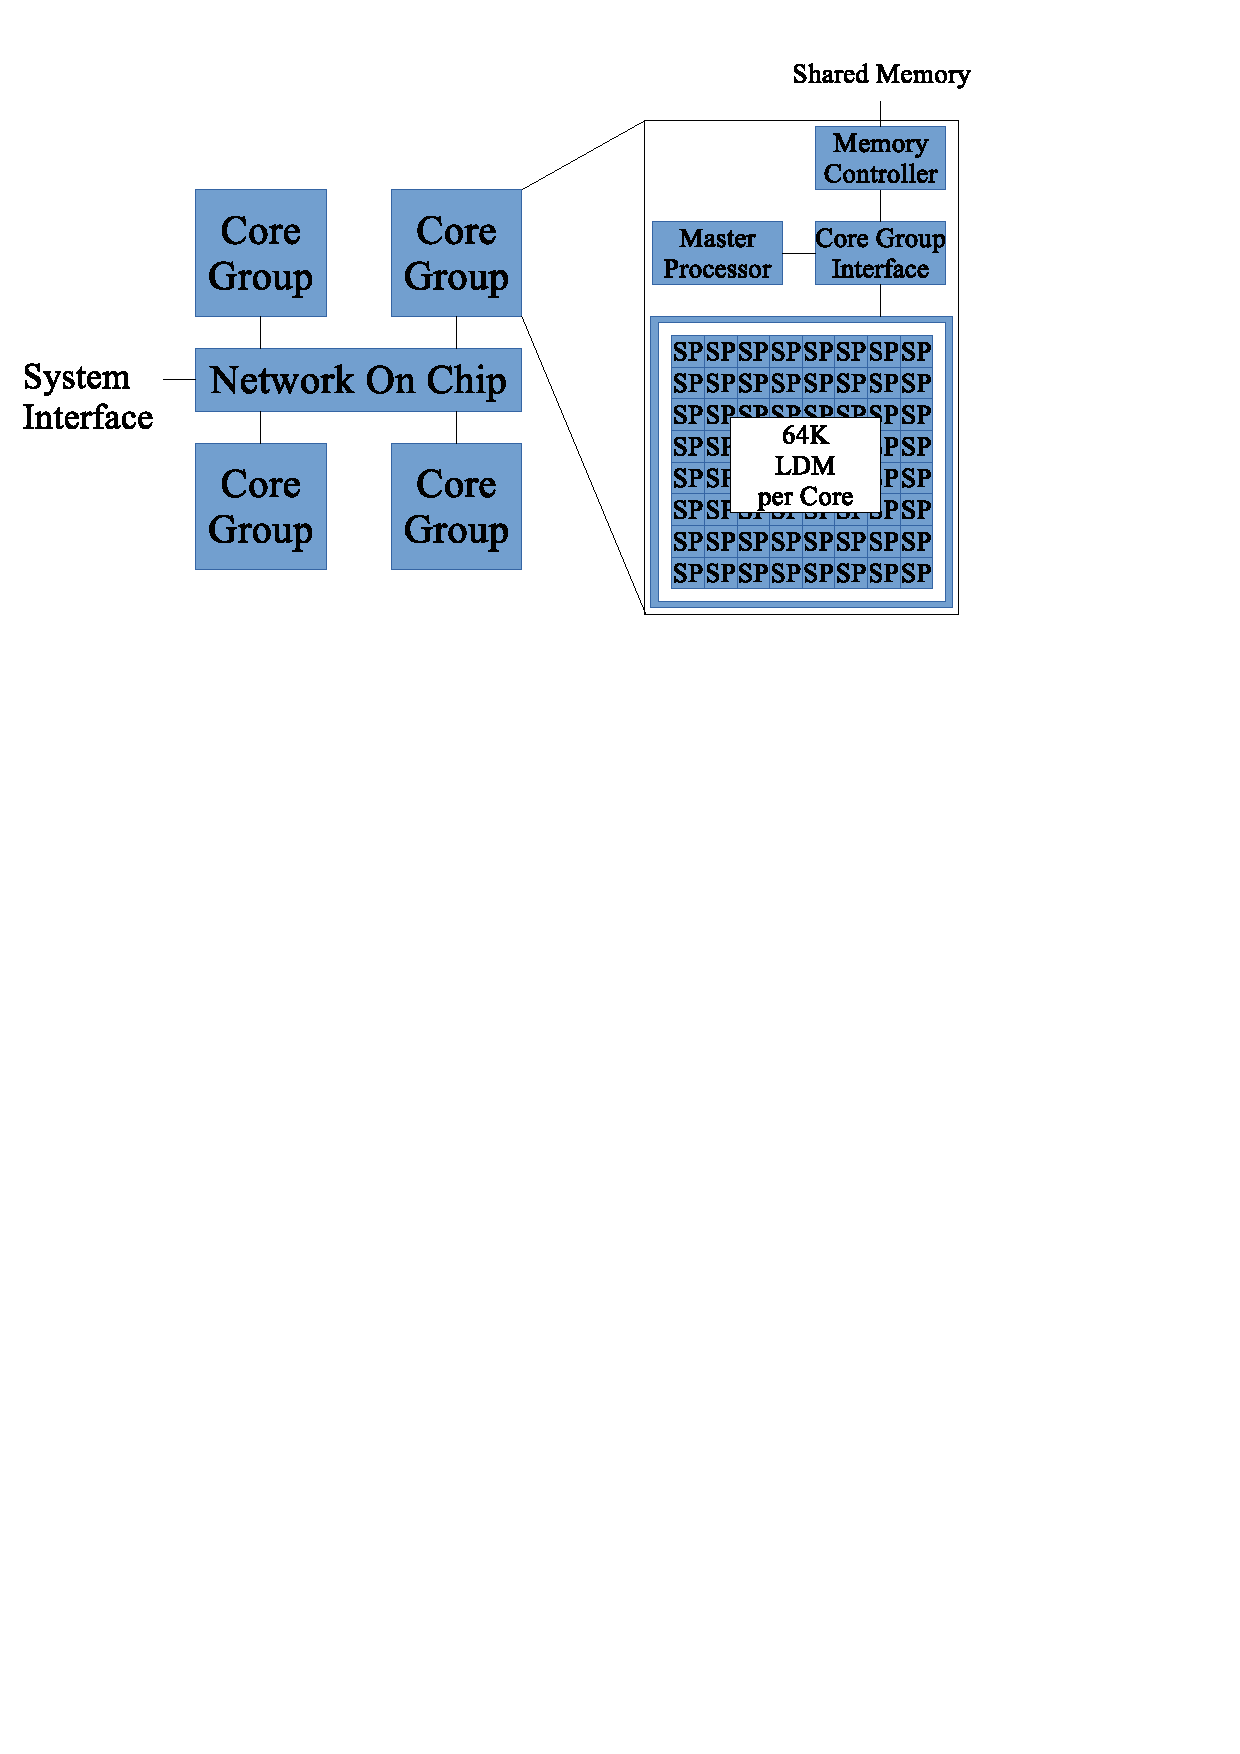
\includegraphics[width=\linewidth]{SW26010}
		\caption{Architecture of the SW26010 processor, which is partitioned into four CGs.}
		\label{fig:SW26010}
	\end{center}
\end{figure}

Each node is equipped with a single SW26010 processor that is subdivided into four {\em compute groups} (CGs). A CG is the basic unit that can be addressed by the job scheduling system. Each CG consists of a single {\em master processor} (MP), 64 {\em slave processors} (SPs), and 8 GB of attached DDR3 shared memory. All nodes can access a shared network file system for loading and storing data. The operating system is a customized Linux flavor running on the MP.  Users may manually launch threads on the SPs in order to parallelize compute-heavy portions of their code. Both the MP and 64 SPs support ShenWei's RISC basic instruction set, which provides scalar and SIMD operations. Moreover, compare and reduction primitives can be called exclusively on the MP, while the SPs exhibit specialized intrinsics for high-precision integer arithmetic. The 8 GB attached shared memory can be accessed by both the MP and the 64 SPs via a memory controller with a shared bandwidth of approximately 136 GB/s. The MP has its own cache (L1 and L2), and each SP can access 64 KB of fast {\em local device memory} (LDM). Data residing in shared memory can be written to LDM using DMA intrinsics and subsequently communicated via a broadcast to the LDM of other SPs. Figure~\ref{fig:SW26010} shows the described hardware layout.

ShenWei's SIMD instruction set features 256-bit wide vector types and a set of corresponding intrinsics provided by the \emph{ShenWei 5 Compiler Collection}.  The MPI library (Sunway MPI) is a derivative of the MPICH implementation, and is compliant with the MPI-3 standard.  Basic threading capabilities for the SPs are provided by the \emph{athread} library.

Previous algorithms mapped onto this novel supercomputer have focused mainly on application domains outside bioinformatics, such as Earth system modeling, ocean surface wave modeling, atomistic simulation, and phase-field simulation \cite{sunway}.

\subsection{Related Work}
There have been a lot of efforts to accerleate read mapping problem on clusters. Among the earliest tools are pBWA \cite{pbwa} and pMap \cite{pmap}. pBWA is an MPI implementation of Version 0.5.9 of the BWA aligner while pMap provides an MPI-based framework for the concurrent execution of popular aligners such as BWA \cite{bwa} and Bowtie \cite{bowtie}. Most of other implementations exploit MapReduce frameworks, for example, the Hadoop-based SEAL \cite{seal} and BigBWA \cite{bigbwa} tools or the Spark-based SparkBWA suite \cite{sparkBWA}, in order to guarantee fault tolerance. Unfortunately, all these approaches suffer from insufficient scalability when scaling to hundreds of nodes. The metaframework parSRA \cite{parSRA} is designed for read mappers written in UPC++.  It combines dynamic scheduling and a virtual file system layer for read distribution to overcome the limitations imposed by pMap and MapReduce-based approaches. merAligner \cite{merAligner} and CUSHAW3-UPC++ \cite{cushaw3upc} are other PGAS-based short-read aligners written in UPC++; both demonstrate good scalability on thousands of cores. Although pMap and parSRA allow for the execution of single node GPU aligners such as nvBowtie \cite{nvBio}, none of the cited tools is explicitly designed for heterogeneous clusters consisting of millions cores. Furthermore, all previous approaches target traditional hardware architectures. 


\subsection{Seed-and-Extend approach}
%There are some "all" mappers currently on traditional commercial platforms, RazerS3\cite{razers3} is one of the most famous "all" mapper on x86\_64 CPUs. Hobbes2\cite{hobbes2}, BitMapper \cite{bitmapper} and mrFAST\cite{mrfast} are also read mappers in "all" mode on x86\_64 platforms. BitMapper2 also supports CUDA-enabled GPUs.

Consider a set of reads ${\cal R}$, a reference genome $G$, and an edit distance threshold $e$. The all-mode read mapping problem can be defined as follows: Find all substrings $g$ of $G$ whose edit distance to some read $R \in {\cal R}$ are no more than $e$. We call such occurrences $g$ in $G$ matches.

This problem can be solved by a classical {\em dynamic programming} (DP) approach that calculates the semi-global alignment between each $R \in {\cal R}$ and $G$. Unfortunately, each alignment results in a time complexity proportional to the product of the sequences' lengths, which renders intractable the alignment of a large number of short reads to a reference genome a few billion letters long.  In order to address this problem, most state-of-the-art solutions \cite{Reinert} employ the {\em seed-and-extend} approach, which follows a three-stage pipeline.

\begin{description}

\item[Stage 1: Filtration.] This stage identifies promising candidate intervals from $G$ (called {\em seeds}) for each read. A popular strategy in order to discard large intervals of $G$ is based on the fact that if a read $R \in {\cal R}$ is divided into $e+1$ non-overlapping $q$-grams (substrings of length $q = \lfloor \lvert R\rvert\ /(e+1) \rfloor$), then (according to the pigeonhole principle) at least one of them occurs exactly in a match. Such occurrences can be identified quickly by looking them up in precomputed $q$-gram index data structure (also called the {\em reference genome index}), which stores all substrings of length $q$ of $G$.

\item[Stage 2. Verification.] This stage determines whether a seed can actually be extended to a full match within edit distance threshold $e$. This requires the implementation of a {\em verification} algorithm in order to analyze the vicinity of each seed. Most mappers typically apply fast versions of DP-based algorithms for this step.

\item[Stage 3. Alignment.] This stage generates the base-pair level alignment information of a read and its verified intervals in $G$. 
%{\color{red} Note that some mappers just use a traceback of Myers delta matrix and some use Smith-waterman, so we shouldn't mention the algorithm}
\end{description}

Established all-mappers such as RazerS3 \cite{razers3} and mrFAST \cite{mrfast} also follow this pipeline. Our profiling of RazerS3 and mrFAST using a typical benchmark data set including the human reference HG19 and 1 million simulated Illumina reads (with a read length of 100 bps) reveals that Stage 2 occupies 67\% and 93\% of the overall runtime, respectively. This shows that a fast implementation of Myers' bit-parallel algorithm for computing the edit distance between a read and an interval is a crucial component when designing efficient all-mappers. 

Consider two strings $s$ and $s \prime$ of length $n$ and $m$, respectively. Their {\em edit distance} is the minimum number of point mutations (i.e. insertions, deletions, or substitutions) required to transform $s$ into $s \prime$. It can be determined by relaxing the cells of a cost matrix $C$ of size $(n+1) \times (m+1)$ according to the recurrence relation shown in Equation~\ref{update_scheme}, where $0 < i \le n$ , $0 < j \le m$ and the {\em characteristic function} $\chi (x \ne y)$ is 1 if $x \ne y$, and 0 otherwise. Initial conditions are set to $C[i,0] = i$, $C[0,j] = j$, and $C[0,0] = 0$. 

\begin{align} \label{update_scheme} 
C[i,j]=\min \begin{cases} C[i-1,j-1]+\chi(s_{i-1} \neq s'_{j-1})\\
C[i-1,j]+1 \\
C[i,j-1]+1
\end{cases}
\end{align}

Myers proposed a bit-vector algorithm \cite{myers} that exploits bit parallelism by encoding the differences (deltas) between adjacent rows and columns in the cost matrix $C$ as defined in Equation~\ref{delta_update}, where $\varDelta h_{i,j}$,  $\varDelta v_{i,j}$, and  $\varDelta d_{i,j}$ are the discrete derivatives of $C[i, j]$ in the horizontal, vertical, and diagonal direction, respectively.

\begin{align} \label{delta_update}
\varDelta v_{i,j}&=C[i,j]-C[i-1,j]   &&\in \{0, \pm1\} \nonumber\\
\varDelta h_{i,j}&=C[i,j]-C[i,j-1]   &&\in \{0, \pm1\} \\
\varDelta d_{i,j}&=C[i,j]-C[i-1,j-1] &&\in \{0, +1\}   \nonumber
\end{align}

Note that the absolute values in Equation~\ref{delta_update} are either 0 or 1. Thus, we can encode the relatively small state space with the help of five vectors using one-hot encoding. Figure~\ref{BitDP} shows an example for the encoding of the vertical derivative $\varDelta v$ and its associated one-hot representations $V^+$ and $V^-$.  With this bit-vector representation the cell updates can be rewritten in terms of logical operations as shown in Equation~\ref{one-hot-myers} \cite{myers}:

\begin{alignat}{100} \label{one-hot-myers}
H^-_{i, j} &= \chi(\varDelta h_{i, j} &&= -1)            &&= V^+_{i, j-1} &&\land D^0_{i, j} \nonumber\\
V^-_{i, j} &= \chi(\varDelta v_{i, j} &&= -1)            &&= H^+_{i-1, j} &&\land D^0_{i, j} \nonumber\\
H^+_{i, j} &= \chi(\varDelta h_{i, j} &&= +1)            &&= V^-_{i, j-1} &&\lor \lnot(V^+_{i, j-1} \,\lor D^0_{i, j}) \\
V^+_{i, j} &= \chi(\varDelta v_{i, j} &&= +1)            &&= H^-_{i-1, j} &&\lor \lnot(H^+_{i-1, j}   \lor D^0_{i, j}) \nonumber\\
D^0_{i,j}  &= \chi(\varDelta d_{i, j} &&= \phantom{+}0)  &&= V^-_{i, j-1} &&\lor H^-_{i-1, j} \lor \chi(s_{i-1} = s'_{j-1}) \nonumber 
\end{alignat}

\begin{figure}[!htb]
	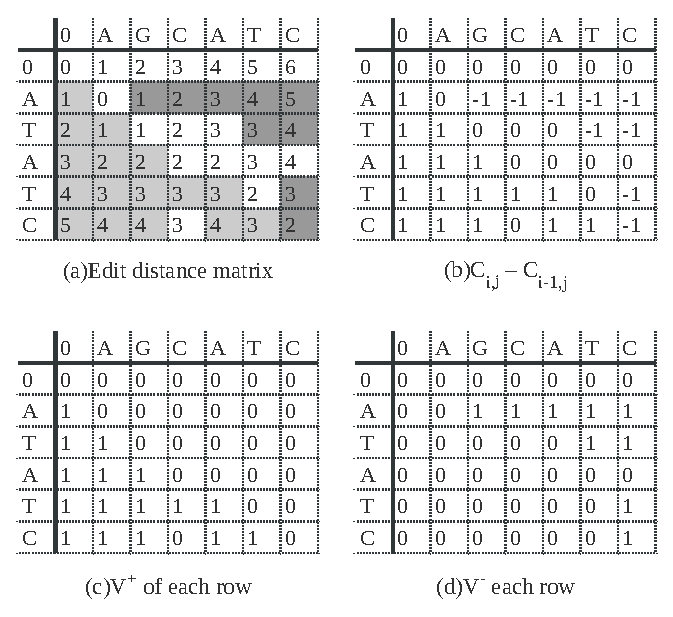
\includegraphics[width=1\linewidth]{BitDP}
	\caption{Relations between the original matrix, $\varDelta v$, $V^+$, and $V^-$.  Here (a) shows the original score matrix; light-shaded cells indicate $\varDelta v_{i,j}=+1$ while heavily shaded cells correspond to $\varDelta v_{i,j}=-1$. The vertical derivative $\varDelta v$ shown in (b) is subsequently one-hot encoded by the bit vectors $V^+$ and $V^-$ in (c) and (d), respectively.}
	\label{BitDP}
\end{figure}


\section{Design of S-Aligner}
\label{Implementation}

This section describes the implementation of both the inter-CG and intra-CG  parallelism for the S-Aligner. Also discussed is our bit-level encoding strategy and the exploitation of local device memory.

\subsection{Large-Scale Inter-CG Parallelization}

\begin{figure}[!htb]
	%\begin{center}
	\includegraphics[width=\linewidth]{GridNew}
	\caption{Our task-partitioning and file-loading strategy: (a) overall design; (b) and (c) detailed behavior of processes.}
	\label{TaskGrid}
	%\end{center}
\end{figure}

The highest level of parallelization employs a coarse-grained partitioning scheme over a block distribution of reads and reference genome using MPI. {\color{red} Weiguo suggests not to mention data size here.} To reduce the excessive data replication of the reference genome index, we employ a partitioning strategy based on a {\em task grid pattern} for the inter-CG parallelization by concurrently assigning pairs of reference genome blocks and read chunks to individual CGs. The two dimensions of the grid are spanned by the reference block identifiers (rows) and read chunk identifiers (columns) as shown in Figure \ref{TaskGrid}(a). Thus, processes in the same row share a unique reference genome (index) block while processes within a column use the same read chunk. Each process executes several cells in one row in order to avoid replication of the relatively big reference index. 

\begin{figure}[!htb]
	\begin{center}
		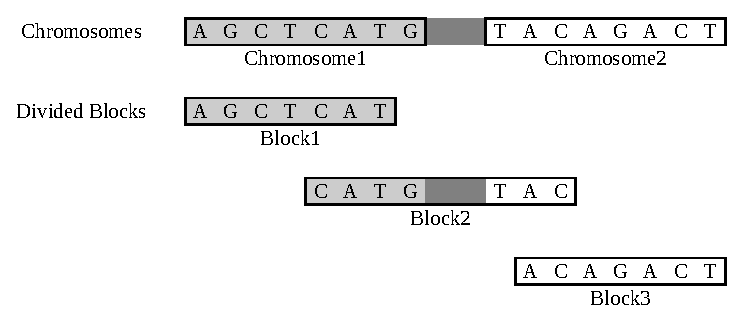
\includegraphics[width=0.9\linewidth]{RefDiv}
		\caption{Exemplary partitioning of a reference genome based on concatenation and padded splits.}
		\label{RefDiv}
	\end{center}
\end{figure}

The read input file is partitioned into chunks of fixed size. This can be easily achieved by splitting by lines. For the reference genome, we first concatenate the individual chromosomes to form one long string. We then divide it into blocks of suitable size according to the memory capacity of a CG ($\approx$300 million bps per block). Note that this partitioning scheme is disadvantageous when a chromosome is scattered over two blocks or a read is mapped to the junction point of two chromosomes. This issue can be resolved by padding `N's between chromosomes. Moreover, when dividing a chromosome into two blocks, we store several base pairs in a neighborhood around the break point in both chunks. As a result, a read is always mapped correctly to a contiguous region. Figure~\ref{RefDiv} depicts this approach.

The computing nodes of Sunway Taihu Light are connected to a network file system via a 1 GBit/s interface, while the overall file system bandwidth is $\sim290$ GB/s for the whole cluster. In practice, efficient data distribution patterns have to be employed to reach reasonable performance. The file system bandwidth is low compared with the bisection bandwidth of $\sim70$ TB/s among compute nodes. To address this issue, we employ a {\em group-and-broadcast} data reuse strategy to avoid redundant file system accesses by sharing identical data via Sunway's network among nodes. As tasks are assigned to grid cells, we cluster processes working on the same reference genome block to a row group ({\em ref broadcast group}), while processes working on the same read chunk are clustered to a column group. If a process calculates cells in the first row or first column ({\em read broadcast group}), it loads the corresponding reference block or read chunk from the file system as shown in Figure~\ref{TaskGrid}(b). Subsequently, it broadcasts the loaded data to processes calculating the same row or column, while the other processes wait for the broadcast data as shown in Figure~\ref{TaskGrid}(c). After the data-loading stage, processes can perform their computation concurrently.

\begin{figure}[!htb]
	%\begin{center}
	\includegraphics[width=\linewidth]{AsyncRead}
	\caption{Asynchronous data loading strategy: (a) default case, and (b) case when there is no significantly shorter reference block.}
	\label{AsyncRead}
	%\end{center}
\end{figure}

Our reference genome partitioning strategy illustrated in Figure~\ref{RefDiv} often generates one reference genome block that is significantly shorter than the others. This block is assigned to the first row of our task grid. Thus, processes in the first row take less time during computation and will have sufficient time to load reads for the subsequent round of computation. This approach therefore reduces the idle time of other processes waiting for read data.  Figure \ref{AsyncRead}(a) illustrates this strategy.

We further provide an optional asynchronous data-loading option in case that there is no significantly shorter reference block. In this case we add a row of processes that loads only reads. When other processes in the column are computing alignments, these processes just load new read chunks. After loading and computation have been completed, all processes within a column receive the loaded data by means of an MPI\textunderscore Bcast. In our experiments, this approach  reduces by over 90\% the idle time between computing two read chunks when using 8 processes.  Figure \ref{AsyncRead}(b) illustrates this strategy.

\subsection{Multithreaded Intra-CG Parallelization}

\begin{figure}[!htb]
	%\begin{center}
	\includegraphics[width=1\linewidth]{FrmWk}
	\caption{Workflow of S-Aligner on a single CG: gray boxes correspond to tasks assigned to SPs while tasks in white boxes are executed on the MP.}
	\label{FrmWk}
	%\end{center}
\end{figure}

The second level of parallelism exploits the threading capabilities of a CG. Our design within a single node is a comprehensive read mapper based on the described seed-and-extend approach using the three-stage pipeline: filtration, verification, and alignment. The filtration step uses a look-up table of $q$-grams of the assigned reference genome block that can be loaded from a preprocessed index file or alternatively calculated on the fly by a radix sort-based hash table construction method. After the MP performs the lookup of each non-overlapping $q$-gram of a read, it stores the retrieved intervals in a SIMD-friendly manner allowing for efficient vectorization during the subsequent verification step on the SPs. Verification selects all intervals that comply with the restricted edit distance using Myers' bit-parallel algorithm. Afterwards, we employ a banded version of the Smith-Waterman algorithm on the SPs to align the remaining intervals that have passed verification. Figure~\ref{FrmWk} shows the workflow of our intra-CG implementation.

\begin{figure}[!htb]
	%\begin{center}
	\includegraphics[width=1\linewidth]{AsyncPara}
	\caption{Asynchronous filtration.}
	\label{AsyncPara}
	%\end{center}
\end{figure}

The intra-CG parallelization is realized by a task parallelization scheme implemented using spawn and join calls of the {\em athread} library. The MP executes the filtration stage while the SPs process the verification step. Each read is divided into non-overlapping $q$-grams. The MP looks up those $q$-grams in the reference genome index and returns a number of intervals. The MP copies them to a buffer that is transferred to the LDM of SPs for verification. We employ a dual buffer strategy by allocating two buffers for storing the intervals identified by the MP. When the MP has finished filling one buffer, it waits for the SP thread group to join, and then dispatches an SP thread group to verify these intervals. Subsequently, the MP fills another buffer, while the SP thread group performs verification. These steps are repeated until all reads are processed (see Figure \ref{AsyncPara}). The dual buffer strategy reduces the idle times of SPs and is also used for implementing the subsequent alignment stage.

\begin{figure}[!htb]
	%\begin{center}
	\includegraphics[width=\linewidth]{SPParallel}
	\caption{Framework of our parallelization scheme within one CG: the MP performs filtration and output of alignment results while SPs verify identified candidate locations and generate base-pair level alignments. Gray boxes indicate the intervals verified in the second round of verification (assuming $slice\_num = 4$).}
	\label{SPParallel}
	%\end{center}
\end{figure}

Figure~\ref{SPParallel} illustrates our framework for dividing the computation between the MP and SPs within a single CG. The number of seeds identified for a given read can vary while the verification time of a single seed is constant. Thus, a simple static assignment of seed intervals per read to SPs can cause workload imbalance.  To balance the workload, we introduce the parameter $slice\_num$, which restricts the maximum number of seed intervals to be verified for one read. If there are more than $slice\_num$ seed intervals to be verified for a read, we spawn verification threads with the first $slice\_num$ intervals. The remaining intervals will be verified in a subsequent round of spawns. A value of $slice\_num$ that is too large can reduce the overhead of spawning SP thread groups, but it worsens workload balance, and vice versa. Our default value of $slice\_num = 100$ provides a good trade-off in practice.

%In our experiments, the dual buffer strategy shows a performance improvement between 50\% to 70\% in the verification stage by minimizing the idle times of SPs. This optimization technique is also used for the alignment stage.

%\subsection{Using Intrinsics}

\subsection{SIMD Vectorization}
Implementing Myers' bit-parallel algorithm using ShenWei's SIMD intrinsics requires a bit-level encoding of DNA sequences to efficiently evaluate the characteristic function $\chi(s_{i-1} = s'_{j-1})$ for all $i, j$.

Different approaches have been used in existing aligners: ($i$) BWA \cite{bwa} employs an {\em array of structures} (AoS), ($ii$) RazerS3 \cite{razers3} stores a DNA sequence in a profile using one-hot encoding. While the AoS approach is more space-efficient and cache-friendly, the usage of a profile with one-hot encoding supports bit-parallel computation in a more efficient way.  Because of the small size of the LDM and the requirement of bit parallelism, we employ an encoding strategy that combines an AoS with an SoA ({\em structure of arrays}) approach, which we call an AoSoA ({\em array of structures of arrays}). This mixed strategy builds two bit-vectors in an interleaved fashion. Thus, we can fetch the encoded sequence by one DMA-intrinsic and calculate $\chi(s_{i-1} = s'_{j-1})$ in terms of two logical equality operations. Figure~\ref{MixPack}  illustrates the encoding strategy.

\begin{figure}[!htb]
	%\begin{center}
	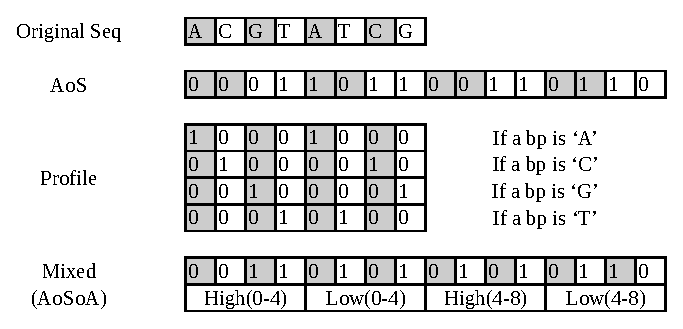
\includegraphics[width=0.9\linewidth]{MixPack}
	\caption{Bit-level encoding strategies for DNA sequences. For simplicity, we use a 4-bit word instead of 64-bit word for illustrating our combined AoSoA strategy (bottom).}
	\label{MixPack}
	%\end{center}
\end{figure}

When updating the five bit-vectors according to Equation~\ref{one-hot-myers} along the columns in a bit-parallel fashion, a circular dependency needs to be resolved: $D^0_{i,j}$ depends on $H^-_{i-1, j}$, which in turn depends on $D^0_{i-1,j}$ (a value we have not computed yet). Myers \cite{myers} has shown that this can be solved by using logical operations and an addition. ShenWei's SIMD instructions support 256-bit integer arithmetic, such as $simd\_uaddo\_take\_carry$ (short for SIMD unsigned octa-word add, taking carry) which adds two 256-bit operands and returns a 256-bit unsigned integer. Thus, different from implementations of Myers' algorithm on other architectures (e.g., \cite{chacon}), our implementation does not require additional instructions to process carries generated within a SIMD lane. Unfortunately, there is no 256-bit compare instruction. Thus, we have implemented comparisons in terms of shifting operations. 

Furthermore, we have simplified the core loop as much as possible in order to avoid branching statements. This action results in an implementation consisting of 23 intrinsics as shown in Figure \ref{cores}, where \texttt{resi32} is set to $|read|\mod 32 - 1$. 

\begin{figure}[!htb]
    \begin{lstlisting}[frame=single, xleftmargin=3.5ex]
t1    = simd_vxorw(ref_hi,read_hi[k]);
t2    = simd_vxorw(ref_lo,read_lo[k]);
X     = simd_vbisw(t1,t2); 
X     = simd_vxorw(X,one); 
X     = simd_vbisw(X,VP[k]);
D0    = simd_vandw(X,VP[k]);
D0    = simd_uaddo_take_carry(D0,VP[k]);
D0    = simd_vandw(D0,VP[k]);
D0    = simd_vandw(D0,X);
HN    = simd_vandw(VP[k],D0);
HP    = simd_vbisw(VP[k],D0);
HP    = simd_vxorw(HP,one);
HP    = simd_vbisw(HP,VN[k]);	
X     = simd_sllow(HP,resi32);
X     = simd_vbisw(X,pr_HP);
pr_HP = simd_srlow(HP,255);
VN[k] = simd_vandw(X,D0);
VP[k] = simd_vbisw(X,D0);
VP[k] = simd_vxorw(VP[k],one);
t2    = simd_sllow(HN,resi32);
t2    = simd_vbisw(t2,pr_HN);
pr_HN = simd_srlow(HN,255);
VP[k] = simd_vbisw(t2,VP[k]);	
    \end{lstlisting}
%	%\begin{center}
%	%{\scriptsize
%	{\footnotesize
%		\begin{tabular}{| l |}\hline
%			\begin{minipage}{0.95\hsize}
%				\verb| |\\
%				\verb|  |~~1. 	t1 = simd\_vxorw(ref\_hi,read\_ hi[k]);\\
%				\verb|  |~~2.	t2 = simd\_vxorw(ref\_lo,read\_ lo[k]);\\
%				\verb|  |~~3. 	X = simd\_vbisw(t1,t2); \\
%				\verb|  |~~4.   X = simd\_vxorw(X,one); \\
%				\verb|  |~~5.  	X = simd\_vbisw(X,VP[k]); \\
%				\verb|  |~~6.  	D0 = simd\_vandw(X,VP[k]); \\
%				\verb|  |~~7.   D0 = simd\_uaddo\_take\_carry(D0,VP[k]); \\
%				\verb|  |~~8.   D0 = simd\_vandw(D0,VP[k]);\\
%				\verb|  |~~9.  	D0 = simd\_vandw(D0,X);\\
%				\verb|  |~10. 	HN = simd\_vandw(VP[k],D0); \\
%				\verb|  |~11.   HP = simd\_vbisw(VP[k],D0); \\
%				\verb|  |~12.  	HP = simd\_vxorw(HP,one);\\
%				\verb|  |~13.   HP = simd\_vbisw(HP,VN[k]);\\	
%				\verb|  |~14.	X = simd\_sllow(HP,resi32);\\
%				\verb|  |~15.   X = simd\_vbisw(X,pre\_HP);\\
%				\verb|  |~16.	pre\_HP = simd\_srlow(HP,255); \\
%				\verb|  |~17.	VN[k] = simd\_vandw(X,D0);\\
%				\verb|  |~18.	VP[k] = simd\_vbisw(X,D0); \\
%				\verb|  |~19.	VP[k] = simd\_vxorw(VP[k],one);\\
%				\verb|  |~20.	t2 = simd\_sllow(HN,resi32);\\
%				\verb|  |~21.	t2 = simd\_vbisw(t2,pre\_HN); \\
%				\verb|  |~22.	pre\_HN = simd\_srlow(HN,255);\\
%				\verb|  |~23.	VP[k] = simd\_vbisw( t2 ,VP[k]);\\	
%			\end{minipage}\\
%			\hline
%		\end{tabular}
%	}
%	%\end{center}
	\caption{SIMD core instructions used to implement Myers' algorithm on ShenWei. The reference sequence is presented as \texttt{ref\_hi}, the high-bit of the pattern, and \texttt{ref\_lo}, the low-bit of the pattern. The read sequence is stored in the vectors \texttt{read\_hi[k]} and \texttt{read\_lo[k]}. The variables \texttt{D0}, \texttt{HN}, \texttt{HP}, \texttt{VN}, \texttt{VP} refer to the corresponding variables in Equation~\ref{one-hot-myers}.}
	\label{cores}
\end{figure}

\subsection{Exploiting Local Device Memory}

\begin{figure}[!htb]
	%\begin{center}
	\includegraphics[width=1\linewidth]{AsyncTrans}
	\caption{Asynchronous data transfer to LDM.}
	\label{AsyncTrans}
	%\end{center}
\end{figure}

Since SPs do not have any cache and the latency to access the DDR3 shared memory is high, the usage of the explicitly managed LDM is crucial.  DMA fetching is the most efficient way to transfer data between main memory and LDM (i.e., significantly faster than using functions such as {\em memcpy}). DMA calls are handled by the memory controller, and SPs can continue to perform computation. Thus, we can overlap data transfers from shared memory to LDM and the verification of intervals using Myers algorithm by using asynchronous DMA-fetching intrinsics presented by ShenWei.

Figure \ref{AsyncTrans} shows our framework for asynchronous data transfer from DDR3 shared main memory to the LDM of SPs. We allocate two buffers in LDM. When an interval in one buffer is verified, the subsequent interval is being fetched to the other buffer using DMA intrinsics. The SP busy-waits for the completion of DMA-fetching before it starts the next verification.

Here we use a busy-waiting strategy because the time used for DMA fetching is usually shorter than the time required for verification. Thus, in the common case the DMA reply word needs to be checked just once in order to pass the busy-wait loop. Our experimental results show that our asynchronous data transfer implementation can almost hide the DMA-fetching latency completely and gains a performance improvement of a factor of 22 compared with an implementation based on {\em memcpy}.

\section{Performance Evaluation}
\label{Evaluation}
The performance of S-Aligner has been evaluated on the Sunway Taihu Light supercomputer. We use GRCh38\footnote{available at http://hgdownload.cse.ucsc.\\edu/downloads.html} as the human reference genome.  For the read input data sets we use either ERR013135\footnote{available at ftp://ftp.sra.ebi.ac.uk/vol1/fastq/ERR013/\\ERR013135} or reads simulated by Mason \cite{mason} or wgsim \cite{wgsim}.\footnote{Note that Mason usually generates reads of higher quality but does not support long reads.}  We first evaluate the performance in terms of runtime and mapping accuracy on a single node. Subsequently, we evaluate the scalability of our implementation by varying the number of utilized nodes up to 13,312.  

\subsection{Single-Node Performance Analysis}

In this experiment, we used the first chromosome of GRCh38 as reference and 20K reads of length 200 bps generated by Mason as input data. 

First, we evaluated the runtime performance of four different implementations of edit distance calculation using Myers' algorithm in one CG: (1) a na\"ive method using the MP only, (2) a na\"ive method with a non-vectorized SP parallelization, (3) a vectorized Myers' algorithm with the MP only, and (4) our vectorized Myers' algorithm with SP parallelization. 

\begin{figure}[!htb]
	\begin{center}
		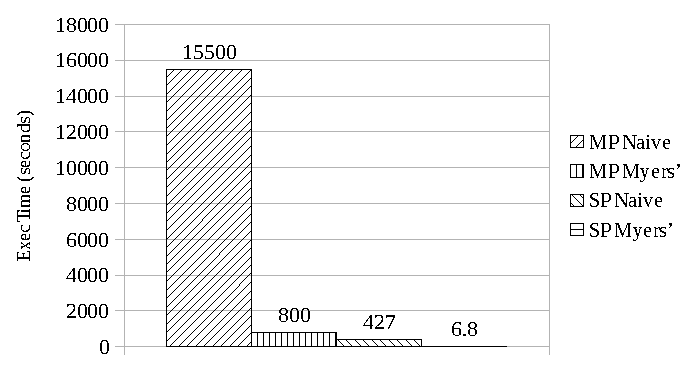
\includegraphics[width=1\linewidth]{VarVerCha}
		\caption{Comparison of the runtimes of four implementations of Myers' algorithm on a single CG.}
		\label{VarVerCha}
	\end{center}
\end{figure}

The result shown in Figure \ref{VarVerCha} demonstrates that making full use of SPs and bit-parallel SIMD vectorization gains dramatic speedups (118$\times$ and 63$\times$, respectively). Since the MP does not support high-precision (256-bit integer) extensions, we implemented a workaround for the high-precision addition operation. This makes it run slower on a single MP than on a single SP. Thus, using SPs can gain a superlinear speedup in this application. Furthermore, our bit-parallel SIMD implementation is able to update 256 cells simultaneously using 23 instructions (i.e., 0.09 instructions per cell) while the na\"ive implementation computes one cell using 6 instructions. This results in a theoretical speedup of $\sim$67$\times$, which explains the actually achieved speedup of 63$\times$.

Second, we evaluated the impact of using asynchronous filtration and the impact of using DMA intrinsics versus memcpy. The result is shown in Figure \ref{VarOptCha}.

\begin{figure}[!htb]
	\begin{center}
		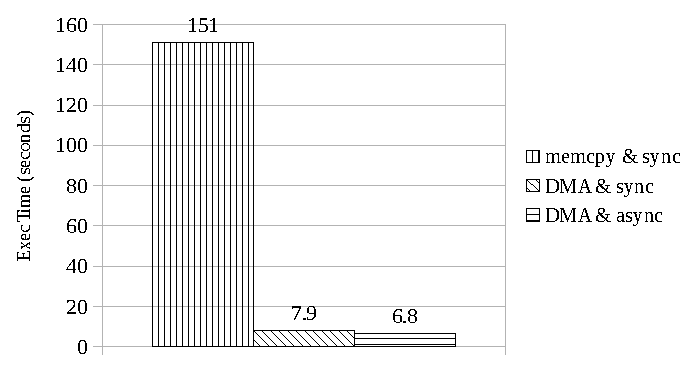
\includegraphics[width=1\linewidth]{VarOptCha}
		\caption{Evaluation with and without I/O optimizations.}
		\label{VarOptCha}
	\end{center}
\end{figure}

The result demonstrates that DMA fetching is key for achieving high performance when using SPs, since a speedup of $\sim$22$\times$ is gained over memcpy. This can be attributed to two factors: (1) DMA transfers require fewer compute resources since they are performed by the memory controller, whereas memcpy uses an SP to write data to memory; (2) DMA fetching can be performed asynchronously, thus enabling the latency of fetching data to be hidden by computation. Furthermore, asynchronous filtration gains $\sim$15\% speedup.

In summary, the architecture of SW26010 differs significantly from a conventional x86\_64 CPU. Straightforward migration of code therefore typically results in an inefficient implementation on SW26010, and architecture-specific optimizations are required in order to achieve high performance. As a case study, we compiled and executed multithreaded BWA \cite{bwa} (one of the most well-known {\em any-best mappers}) on SW26010. It runs two times slower than S-Aligner, while finding significantly fewer locations, showing the importance of making changes according to this specific architecture.

\subsection{Comparison with RazerS3}
In this experiment, we use the first chromosome from GRCh38 as reference and various number of reads from ERR013135. The runtime of S-Aligner on a single SW26010 node is compared with RazerS3, a representative all-mapper. Since RazerS3 does not support ShenWei's architecture, we ran it on a machine with Intel processors using multithreading with default parameters (e.g., the accuracy parameter is set to 98\%). Measured runtimes are shown in Table \ref{SingleNode}.  One can see that S-Aligner executed on a single SW26010 (260 cores running at 1.45 GHz) outperforms RazerS3 running on eight Xeon E7-8860v3 CPUs (128 cores running at 3.2 GHz).

\begin{table}
	\begin{threeparttable}
		\caption{Runtime comparison between S-Aligner running on a single CG and RazerS3 running on a single node with eight Xeon E7-8860v3 CPUs.}
		\label{SingleNode}
		\begin{tabular}{@{\extracolsep{2pt}}rrrrr}
			\hline
			\multicolumn{1}{c}{Ref} &
			\multicolumn{2}{c}{Reads} &
			\multicolumn{2}{c}{Time(s)}\\
			\cline{2-3}
			\cline{4-5}
			\multicolumn{1}{c}{\#bps} &
			\multicolumn{1}{c}{Count} &
			\multicolumn{1}{c}{\#bps} &
			\multicolumn{1}{c}{RazerS3\tnote{\textdagger}} &
			\multicolumn{1}{c}{S-Aligner\tnote{\textdaggerdbl}}\\
			\hline
			%65M & 10M  & 108 &  52\tnote{\textdagger} & 47\tnote{\textdaggerdbl}\\
			%58M & 40M  & 108 &  1415 & 435\\
			116M & 40M & 108 &  939 & 405\\
			253M & 40M & 108 &  3,044 & 892\\
			%58M & 40M  & 200 &  898 & 1,002\\
			%116M & 40M & 200 &  744 & 1,013\\
			253M & 40M & 200 &  3,430 & 2,580\\
			\hline
		\end{tabular}
		\begin{tablenotes}
		\item[\textdagger] result is from a machine with eight Xeon E7-8860v3 (128 cores up to 3.20GHz).
		\item[\textdaggerdbl] result is from a node with a SW26010 (260 cores with frequency of 1.45GHz). 
		\end{tablenotes}
	\end{threeparttable}
\end{table}

Rabema \cite{rabema} (Read Alignment BEnchMark) is a well-defined read alignment benchmark that can evaluate the quality of read mappers in both {\em all} and {\em any-best} mode. We evaluated the accuracy of S-Aligner in all mode based on Rabema by using the result of RazerS3 with the accuracy parameter set to 100\% as gold standard. S-Aligner can find up to 99.8\% of the normalized intervals found by RazerS3 (100\% accuracy), which is higher than the accuracy of RazerS3 executed with default parameters (98\% accuracy). Detailed results are provided in Table~\ref{AccuEval}.

%As we can see, our algorithm has better performance than RazerS3, with an accuracy no worse than ordinary RazerS3.

\begin{table}
	\begin{threeparttable}
		\caption{Accuracy evaluation of S-Aligner for both real and simulated data.}
		\label{AccuEval}
		\begin{tabular}{@{\extracolsep{2pt}}rrrrrr}
			\hline
			\multicolumn{1}{c}{Chrom} &
			\multicolumn{3}{c}{Reads} &
			\multicolumn{1}{c}{\multirow{2}{*}{Interv. found}} \\
%			\multicolumn{1}{c}{Normalized}\\
			\cline{2-4}
			\multicolumn{1}{c}{Index} &
			\multicolumn{1}{c}{Origin} &
			\multicolumn{1}{c}{Count} &
			\multicolumn{1}{c}{\#bps} \\		
%			\multicolumn{1}{c}{intervals found}}\\
			\hline
			%65M & 10M  & 108 &  52\tnote{\textdagger} & 47\tnote{\textdaggerdbl}\\
			%58M & 40M  & 108 &  1415 & 435\\
			1\textsuperscript{st} & ERR013135 & 20,000 & 108 & 99.34\%\\
			1\textsuperscript{st} & Mason &  20,000 & 200 & 99.82\%\\
			\hline
		\end{tabular}
	\end{threeparttable}
\end{table}

\subsection{Scalability Analysis}

To evaluate weak and strong scalability, we measured the runtimes of S-Aligner using different numbers of nodes ranging from 13 to 13,312. The full GRCh38 assembly of the human genome was used as reference. Input reads were simulated by Mason with an error rate of 4\% and a length of 200 bps. Weak scalability was measured for numbers of nodes ranging from 13 to 3,328 by increasing the number of input reads from 16 million to 4 billion, correspondingly. Strong scalability was measured by increasing the number of nodes from 3,328 to 13,312 while keeping the number of input reads constant at 4 billion. We measured the performance in terms of {\em read base-pairs processed per second} (bpps) in total and normalized per node (see Table \ref{paraexp}). Figure \ref{VarProcCha} shows the achieved speedups and efficiencies. The results demonstrate weak scalability since the normalized node performance is almost constant for the number of nodes ranging from 13 to 3,328. Furthermore, the node performance only slightly decreases when increasing the number of nodes from 3,328 to 13,312 while keeping the amount of input reads constant at 4 billion, thus demonstrating strong scalability for sufficiently large input datasets.  

\begin{table}[!htb]
	\begin{threeparttable}
		\caption{Performance and runtime evaluation of S-Aligner using different numbers of nodes.}
		\label{paraexp}
		\begin{tabular}{rrrrrr}
			\hline
			\multicolumn{1}{c}{\multirow{2}{*}{\#nodes}} &
			\multicolumn{2}{c}{Reads}  &
			\multicolumn{1}{c}{\multirow{2}{*}{Time(s)}} &
			\multicolumn{2}{c}{Performance (bpps)} \\
			\cline{2-3}
			\cline{5-6}
			\multicolumn{1}{c}{} &
			\multicolumn{1}{c}{Count} &
			\multicolumn{1}{c}{\#bps} & &
			\multicolumn{1}{c}{Total (M)} &
			\multicolumn{1}{c}{Node (K)}\\
			\hline
			13 & 16M & 200 & 1,315 & 2.43 & 185.43\\
			%			26 & 64 & 2664 & 4.9 & 187\\
			52 & 64M & 200 & 1,321 & 9.69 & 184.80\\
			%			104 & 64 & 2664 & 4.9 & 187\\
			208 & 256M & 200 & 1,321 & 38.76 & 184.66\\
			%			416 & 64 & 2664 & 4.9 & 187\\
			832 & 1,024M & 200 & 1,327 & 154.33 & 184.59\\
			%			1664 & 64 & 2664 & 4.9 & 187\\
			3,328 & 4,096M & 200 & 1,349 & 607.26 & 179.67\\
			13,312 & 4,096M & 200 & 344 & 2,381.40 & 178.90\\
			\hline
		\end{tabular}
		\begin{tablenotes}
			\item
			\#nodes is the number of nodes involved in computing.
			\item
			bpps is short for million bp processed per second.
			\item
			M / K indicates that column is presented in millions / thousands.
		\end{tablenotes}
	\end{threeparttable}
\end{table}

\begin{figure}[!htb]
	\begin{center}
		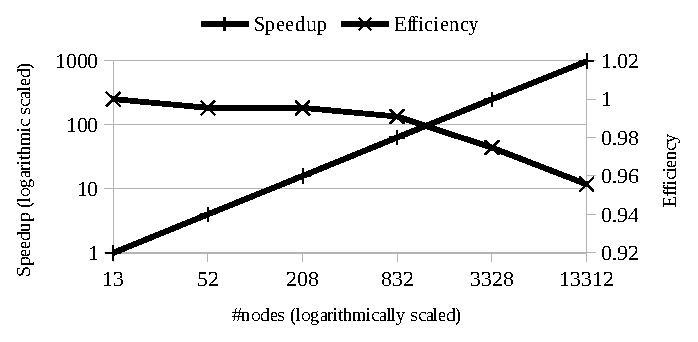
\includegraphics[width=1\linewidth]{VarProcCha}
		\caption{Speedup and efficiency of S-Aligner for different numbers of nodes.}
		\label{VarProcCha}
	\end{center}
\end{figure}



\section{Conclusion}
\label{Conclusion}

NGS data will continue to grow rapidly in the foreseeable future. Read mapping is a critical and compute-intensive step for a variety of NGS pipelines. While significant efforts have been devoted to optimizing this task, it is still a major bottleneck. In this paper, we have introduced S-Aligner---a highly scalable read mapper specifically designed to fit the characteristics of the Sunway Taihu Light supercomputer and its SW26010 architecture.
It scales almost linearly with over 95\% parallelization efficiency when distributed over more than 50,000 processes. As a result, S-Aligner can map $\approx$ 1.6 TB of read data to the whole human genome in just a few minutes. Moreover, when executed on a single node it can outperform the popular all-mapper RazerS3 executed on eight Xeon E7-8860 CPUs while achieving comparable mapping accuracy.

The design of S-Aligner teaches a number of lessons about properly designing parallelization and communication patterns in order to achieve both high performance and scalability on the new Sunway Taihu Light supercomputer. First, both multithreading and SIMD vectorization need to be employed to fully exploit the computational resources of the SW26010 processor. Second, within an SP the fast LDM must be used via DMA intrinsics in order to guarantee efficient intra-CG communication. Third, a scalable inter-CG communication scheme must be implemented in a way that efficiently hides the interconnection network bottleneck. Fourth, asynchronous file-loading and data-sharing strategies need to be implemented in order to effectively hide the latency of the network file system. The techniques presented in this paper could also be adapted to map similar applications exhibiting a pipeline of hashing and verification, such as large-scale approximate near duplicate object detection \cite{efficient} or de novo genome assembly \cite{swap} onto the heterogeneous many-core cluster architecture of Sunway Taihu Light. 

%replace this by a "lessons learned" paragraph for Sunway Taihu Light programming
%Possible directions of future research are 1\textsuperscript{st} the design of a dynamic scheduler based on MPI's one-sided communication primitives to allow for a better load balancing, and 2\textsuperscript{nd} the porting of MP-exclusive tasks to SPs in order to further increase performance.       


\bibliographystyle{plain}
\bibliography{references.bib}
% That's all folks!
\end{document}

%I'm very tired to navigate over the abandon paragraphs in the tex, thus I moved them here or in the version of Dec 18, 10:37pm.

%Formerly in Abstract:
%About the file system:
%Moreover, since each node has a low file system bandwidth but and the file system will have performance down if there are too many requests, so asynchronous access and data sharing strategy are employed during file IO to maximize the bandwidth to the file system.	{\color{red} Xiaohui, further specify the aforementioned sentences, please. You know the bottlenecks best!}

%About arch:
	
% REMARK (Christian): We should move this to the introduction
%The Sunway Taihu Light supercomputer has 40,960 nodes, each node has four computation groups (CG), each of CG has a master processor (MP) and a slave processor (SP) group formed by 64 slave processors, and supports ShenWei's SIMD extension, so we employ a flexible data partition strategy among CGs and a two-level parallelization  strategy in a single CG according to Sunway's architecture, and achieve an efficient utilization of the entire system.
	
%In our implementation, we use MP for lookup works and SP for computation works. The most compute-bounded stage of S-Aligner is the verification of large amounts of potential mapping intervals by Myers algorithm, and we accelerate this stage by using the SP group. Since the memory bandwidth is shared by all processors in one CG, we also use SPs to parallelize a large amount of discrete memory access, also, asynchronous IO strategies are applied to reduce the latency of data transfer.

%Just rewrite:

%Since our algorithm is data-intensive as well, we divide MPI processes to groups with hundreds of processes, and use task grid and group-and-broadcast strategy to transfer shared data, and with the number of nodes grows, our implementation gains almost linear speedup on up to 13,312 nodes with 53,428 processes. 

%Formerly in Introduction:

%With the rapid advance of NGS technology, computational biology has experienced great development, and the NGS technology are now widely applied to various fields including CHIP-seq, RNA expression profiling through RNA-seq, DNA Structural Variation detection, and Genome Assembly.

%The emergence of NGS instruments, such as Pacific Biosciences and Illumina MiSeq sequencers\cite{reviewngs}, can produce billions of short sequence data (reads) with length from 25 to 15,000 base pairs (bp) each in a day. 

%To make use of these reads, the most important and time-consuming step is to map them to a known DNA sequence (reference), generating bp-level alignments between each read and its potential originating region on the reference. Alignment are required by most DNA sequence analysis, such as genotyping, SNP discovery and personal genomics.

%References contain a mass of base-pairs, for example, there are more than 3 billions of bps in one human genome reference, but traditional local comparison algorithms like Smith-Waterman\cite{sw} usually come with quadratic time complexity computing the similarity between a read and all substrings from a reference. Thus applying this kind of algorithms to read mapping can take  several weeks even months if serially processed on a personal computer.

%There are two modes of read mapping: "any-best" mode and "all-best" mode\cite{allany}, for example, Bowtie\cite{bowtie}, Bowtie2\cite{bowtie2}, BWA\cite{bwa} and GEM\cite{gem} run in "any-best" mode, and they try to identify one or a few best mapping intervals for each read, while RazerS3\cite{razers3}, Hobbes2\cite{hobbes2}, BitMapper\cite{bitmapper} and mrFAST\cite{mrfast} run in "all-best" mode, that is, they find all mapping intervals satisfying some constraint (eg. under a restricted edit distance).

%Obviously "any-best" mappers are usually faster than "all-best" mappers, but some researches need the information about all potential originating intervals of a read from a reference genome, for example, it is much easier to study gene innovation and phenotypic variation if a mapping result of an "all-best" mapper is provided. Therefore S-Aligner is developed as an "all-best" mapper, fulfilling requirements of different applications, and it comes with good scalability, so it can be faster than many "any-best" mappers if enough nodes are provided.
%With the explosive growth of sequence data size, some recent sequencing data can make mapper take several days on a workstation-level computer to compute the alignment, so mapping enormous reads has become a challenge in computational biology. Thus, it is essential and practical to port alignment tools to clusters or supercomputers.
%Supercomputers often comes with co-processors like GPU, Xeon Phi or customized ones, and these co-processors often come with significant performance improvement and better energy/cost efficiency in scientific computing. But how to make full use of these co-processors in computational biology becomes a problem.
%Recently released supercomputer Sunway Taihu Light comes with an architecture  like a neo-heterogeneous platform somehow. The Sunway Taihu Light contains 40,960 nodes equipped SW26010 processor, with 163,840 CGs in total, and each CG has one MP and 64 SPs, while both MP and SP from Sunway Taihu Light are compatible to ShenWei's RISC instruction set except some extensions are not available on SP, so it is regarded as a good platform for sequence alignment problem because both MP and SP have a good performance to handle both scalar and vector operations.

%In this paper, we present our work of a fast and efficient read mapper on SW26010 processor with MPI capability, and it has been evaluated on Sunway Taihu Light since biology computing problem is often popular on most highly ranked supercomputers. We introduce an efficient implementation to find all possible intervals within a reference sequence that matches a read with restricted edit distance. In summary, the main contribution of our work are:

%\begin{enumerate}
% 	\item
% 	In the inter CG level, we use MPI technology to make full use of multiple CGs and apply task grid and broadcast in row/column strategy to achieve a balanced workload and efficient parallelization.
% 	\item
% 	In the intra CG level, we use task parallelism in one CG: using MP for reference index lookup and misc operations like IO or data transfer and using the SP group for the most compute-bounded verification and alignment operation, and we use data parallelism multi-threading among SPs.
% 	\item
% 	In the intra SP level, we use ShenWei's SIMD extension to accelerate the Myers algorithm.
% 	\item
% 	Besides, we use many asynchronous strategy to reduce IO overhead, including file reading among CGs, computing between MP and the SP group and task data fetching on SPs, which greatly decreased processors' idle time.
    %\item
    %We implement the Myers' algorithm using SPs and parallelize it using athreads, which is thousands times faster than the single thread naive implementation of edit distance.
	%\item
	%We make use of LDM via DMA-intrinsics, which gains 22 times speed up over the non-DMA implementation.
	%\item
	%We employ efficient inter CG parallelization strategy, and it can achieve an efficiency of over 97\% with 53,248 CGs.
%\end{enumerate}

%\begin{itemize}
%	\item
%	In Section \ref{Related Work}, we introduce some related algorithms, implementations, and the Sunway Taihu Light supercomputer.
%	\item
%	In Section \ref{Implementation}, we present the implementation in detail, including intra SP, intra CG and inter CG optimization.
%	\item
%	In Section \ref{Evaluation}, we show our evaluation results, including single node and mass parallel experiments.
%	\item
%	In Section \ref{Conclusion}, we concludes the paper.
%\end{itemize}

%Formerly in Related work:

%{\color{green} try write something about razers3}

%corresponding intrinsics library is provided by \textit{ShenWei 5 Compiler Collection} (\textit{sw5cc}), and \textit{sw5cc} also contains an MPI runtime compatible with \textit{mpich2-3.04}.

%For supporting SPs, ShenWei provides an \textit{athread} library, which can start threads on SPs, there are mainly two method to start threads in \textit{athread} library, one is \textit{create}, which creates one thread with an optional parameter and bind it to one SP, the other is \textit{spawn}, which creates a thread for each SP, while these threads share an optional parameter.


%\subsection{Pigeonhole Principle}
%{\color{red}
%The number of potentially matching positions in the reference genome can be drastically reduced by applying filters to the candidate set from the seed stage. S-Aligner employs such a preprocessing filter based on the \emph{pigeonhole principle}. To put it in simple words, if $n$ items are put into $n+1$ boxes that one or more boxes must be empty.
%%For sequence alignment problem, we note the reference genome as $ref$ and the read sequence as $read$, and $s[i, j]$ as the substring of string $s$ starting from $i$ with length $j$, then we define $q\_gram$ and $L_q$ as follows:

%In the context of sequence alignment, let us refer to the reference genome as $ref$ and to the read as $read$. Moreover, the contiguous subsequence of the string $s$ starting at position $i$ with length $j$ shall be denoted as $s[i, j]$. Correspondingly, a $q$-gram is defined as strided substring of length $q$: $q\text{-gram}(i) := read[i \cdot q, q]$. Furthermore, let
%%\begin{equation}
% \label{LQ}
% L_q(i):=\{x | ref[x + i \cdot q, q] = q\_gram(i)\} \quad.
% \end{equation}

% Then we divide read into $n=\lfloor \cfrac{|read|}{q}\rfloor$ $q\_gram$s, from $q\_gram(0)$ to $q\_gram(n - 1)$ and $L_q(i)$ is the set of intervals $l$ that if $read$ is mapped to $l$th bp of $ref$, $q\_gram(i)$ will be exactly mapped, additionally, we define $M_e$ is the set of intervals that $read$ can be mapped to with edit distance at most $e$.

% Then if a read can be mapped to a interval on the reference with at most $e$ edits, at least $n - e$ of the non-overlapping q-grams can be mapped to the reference exactly because there are at most $e$ edits, so if $n > e$, we have
% \begin{equation}
% M_e \subseteq \bigcup^{n}_{i=0}L_q(i)
% \end{equation}.

% Moreover, we have
% \begin{equation}
% \label{MeinG}
% M_e \subseteq \bigcup_{i \in G}L_q(i)
% \end{equation}
% for any $G$ that $G \subseteq [0, n) \land |G| > e$ because at least one q-gram can be mapped exactly.

% For reducing the number intervals for further filtration, we may choose the $G$ having minimum
% \begin{equation}
% \sum_{i \in G}|L_q(i)|
% \end{equation}
% . According to (\ref{MeinG}), this can be done by selecting $e + 1$ $L_q$s with minimum $|L_q|$. 

% THE WHOLE SUBSECTION IS BARELY READABLE AND HAS TO BE REVISED THOROUGHLY: BETTER EXPLAIN THE SETS M\_e and L\_q !  
%}
%{\color{green} Weiguo suggests to move this to algorithms section}

%Edit distance is one of the most popular measures for interval verification with restricted number of edit operations $e$. Similar to Smith-Waterman's algorithm, edit distance is computationally demanding since its dynamic programming algorithm exhibits a time complexity proportional to the product of sequence lengths. Let $n$ and $m$ be the lengths of two compared strings $s$ and $s'$ then their edit distance can be determined by relaxing the cells of the $(n+1) \times (m+1)$ shaped cost matrix $C$ according to the recursive scheme
%\begin{equation}
%\delta_{ij}=\left\{
%\begin{array}{rcl}
%0,     &      & {ref\_map_{i}=read_{j}},\\
%1,     &      & {otherwise}\\
%\end{array} \right.
%\end{equation} 
% where $0 < i \le m$, $0 < j \le n$, and the characteristic function $\chi(x \neq y)$ being one for all $x \neq y$ and zero otherwise. 
%It is obviously the time complexity of calculating this DP matrix is $O(n\cdot m)$, as $m$ is often close to $n$, the complexity is also regarded as $O(n^2)$. It is slow to calculate the matrix with a naive recurrence method, but 
% Myers proposed a bit-vector algorithm \cite{myers} that exploits bit parallelism by encoding states in an integer representation. To achieve that the differences (deltas) between adjacent rows and columns in the cost matrix $C$ are used instead of their absolute values. The adjacent encoding reads as follows
% \begin{alignat}{100}
% \varDelta v_{i,j}&=C[i,j]-C[i-1,j]   &&\in \{0, \pm1\} \nonumber\\
% \varDelta h_{i,j}&=C[i,j]-C[i,j-1]   &&\in \{0, \pm1\} \nonumber\\
% \varDelta d_{i,j}&=C[i,j]-C[i-1,j-1] &&\in \{0, +1\}   \quad,
% \end{alignat}
% where $\varDelta h_{i,j}$,  $\varDelta v_{i,j}$ and  $\varDelta d_{i,j}$ are the discrete derivatives of $C[i, j]$ in direction of its left, upper, and diagonal cell. Note that their absolute value is either zero or one due to the uniform choice of gap penalties and substitution costs in Equation~\ref{update_scheme}. As a result, we can encode the relatively small state space with the help of five vectors:
%and the absolute value of them is never greater than 1, and it is proved in \cite{myers}, so we can encode $\varDelta h_{i,j}$,  $\varDelta v_{i,j}$ and  $\varDelta d_{i,j}$ to following bit-vectors:
% \begin{alignat}{100}
% V^\pm_{i,j} &= \chi(\varDelta v_{i, j} = \pm1) \nonumber\\
% H^\pm_{i,j} &= \chi(\varDelta h_{i, j} = \pm1) \nonumber\\
% D^0_{i,j}   &= \chi(\varDelta d_{i, j} = \phantom{\pm}0) 
% \label{one-hot-myers}
% \end{alignat}
%{\color{green} what does $\chi(s_{i-1} \neq s'_{j-1})$ mean, if we can write formulas above like this:
%$$
%V^\pm_{i,j} = \chi(\varDelta v_{i, j} = \pm1)
%$$
%}
%Figure~\ref{BitDP} shows an example for the encoding of the vertical derivative $\varDelta v$ and its associated one-hot representations $V^+$ and $V^-$. Using the bit-vector representation from Equation~\ref{one-hot-myers} the cell updates can be rewritten as follows \cite{myers}:

% \begin{alignat}{100}
% H^-_{i, j} &= V^+_{i, j-1} &&\land D^0_{i, j} \nonumber\\ 
% V^-_{i, j} &= H^+_{i-1, j} &&\land D^0_{i, j} \nonumber\\
% H^+_{i, j} &= V^-_{i, j-1} &&\lor \lnot(V^+_{i, j-1} \,\lor D^0_{i, j})   \nonumber\\
% V^+_{i, j} &= H^-_{i-1, j} &&\lor \lnot(H^+_{i-1, j}   \lor D^0_{i, j})   \nonumber\\
% D^0_{i,j}  &= V^-_{i, j-1} &&\lor H^-_{i-1, j} \lor \chi(s_{i-1} = s'_{j-1})\quad. \label{EVform}
% \end{alignat}

%Formerly in Implementation:

%Afterwards, we hash all 12-mers from the reference to a 24 bit collision-free hash map. The keys are implicitly defined by the slot indices and the values correspond to the interval positions in the reference. Figure~\ref{HIdx} shows the memory organization of the buckets. Multiple values are simply stored in a contiguous 1-d array $hv\_pos$, while another array $hv\_index$ stores the offsets to the buckets. This can be achieved in linear time using default array compaction techniques based on adjacent comparisons, a subsequent prefix scan, and a final substitution phase.

%The resulting index is relatively large. Let $n$ be the length of a chromosome then its concatenated DNA sequence has a length of $2n$. The size of $hv\_pos$ corresponds to $2n\log(2n)$ bits since we need at least $\log(n)$ bits to represent the index space. Analogous, the array of offsets $hv\_index$ occupies $2^{24}\log(2n)$ bits. Note that variable word length may hurt performance and thus we stick to 32 bit integers which is enough for the length of a chromosome.

%This results in an overall size of $(32 \cdot 2n + 32 \cdot 2^{24}) \text{ bits} = (8n+64M) \text{ bytes}$. Thus, for a chromosome of size 300 MB the index occupies roughly 2,464 MB which is more than one-third of the available memory of a CG. Nevertheless, the described data structure exhibits reasonable performance due to its cache-friendly memory layout. 

%Since the alignment generation is less often called than the verification, the efficiency of this stage is less important, we implemented a naive Smith-Waterman algorithm to generate alignments on the SPs with only one optimization: for we just fill cell $(i, j)$ if $|i - j| \leq e$ (where $e$ is the edit distance restriction defined in last subsection), and the time taken by alignment in this step is about 1/1000 of the verification, so this step is less worthy to optimize.

%\subsection{Data Structures}
%\label{DataStructure}

%\subsubsection{Reference Index}
%{\color{green} Weiguo suggests it should be removed}
% We construct a hash index for each reference block mentioned in Section \ref{DataStructure}. In particular, we replace 'N's in the block with random base pairs, and subsequently append the block's reverse complement to the end of this block. As a result, we can stick to the 2 bit encoding of nucleotides and do not have to waste an additional bit for 'N'. Moreover, we can ignore reversed reads during mapping.
% %so that we can use 2 bits to encode a bps and we do not need to reverse reads while computing mapping, and we note the modified sequence as $ref$.

% %Then we hash all 12-mers from the $ref$ to a 24-bit collision-free hash value, and store each k-mer's index on the $ref$ to a bucket corresponding to its hash value, Fig.\ref{HIdx} shows our memory organization of these buckets, we use 1-d array $hv\_pos$ to store elements of the buckets, while another array $hv\_index$ stores the start index of buckets.
% Afterwards, we hash all 12-mers from the reference to a 24 bit collision-free hash map. The keys are implicitly defined by the slot indices and the values correspond to the interval positions in the reference. Figure~\ref{HIdx} shows the memory organization of the buckets. Multiple values are simply stored in a contiguous 1-d array $hv\_pos$, while another array $hv\_index$ stores the offsets to the buckets. This can be achieved in linear time using default array compaction techniques based on adjacent comparisons, a subsequent prefix scan, and a final substitution phase.

% %This can be done by a 2-round scanning of $ref$. In the first round, we count the numbers of k-mers grouping by their hash value, and store them in $hv\_index$, then we do a accumulate sum of $hv\_index$ and determine the index to put elements. In the second round, we put the index of each k-mer on the $ref$ to corresponding position of $hv\_pos$.

% The resulting index is relatively large. Let $n$ be the length of a chromosome then its concatenated DNA sequence has a length of $2n$. The size of $hv\_pos$ corresponds to $2n\log(2n)$ bits since we need at least $\log(n)$ bits to represent the index space. Analogous, the array of offsets $hv\_index$ occupies $2^{24}\log(2n)$ bits. Note that variable word length may hurt performance and thus we stick to 32 bit integers which is enough for the length of a chromosome.
% %, we use 32 bit integer type to store $hv\_pos$ and $hv\_index$,
% This results in an overall size of $(32 \cdot 2n + 32 \cdot 2^{24}) \text{ bits} = (8n+64M) \text{ bytes}$. Thus, for a chromosome of size 300 MB the index occupies roughly 2,464 MB which is more than one-third of the available memory of a CG. Nevertheless, the described data structure exhibits reasonable performance due to its cache-friendly memory layout. 

% %But this index structure achieves a good performance, for each 12-mer from reads, it is only needed an array access to find out the start position of its mapped intervals in the $hv\_pos$, and it is very friendly to the cache of MP since these intervals are stored in a continuous way, and easily coped to buffers for SPs to fetch.
% \begin{figure}[!htb]
% 	\begin{center}
% 		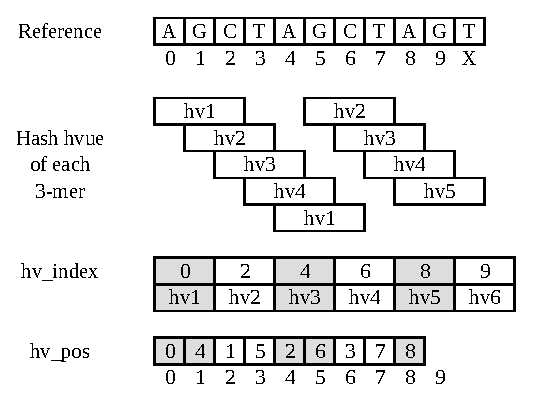
\includegraphics[width=0.9\linewidth]{HIdx}
% 		\caption{Memory layout of the hash index. For the sake of simplicity, we use 3-mers instead of 12-mers.}
% 		\label{HIdx}
% 	\end{center}
% \end{figure}

% \subsubsection{Mixed Sequence Packing}
% {\color{green} Maybe move this to SIMD section}
% In order to efficiently compute the contributions of the substitution term $eq_{i,j}$ (see Section \ref{SecMyers}) we transform both the read and reference into a bit-vector representation. The literature states three major packing strategies: continuous packing, separated packing and one-hot coding. The first one simply stores the sequences in a single bit-vector where the even bits encode the lower and the odd bits the upper part of the 2 bit representation of nucleotides, so to speak, as array of structs (like BWA). The second strategy employs two bit-vectors to separate the even and odd contributions (struct of arrays). The third strategy interprets the four base pairs as class labels and subsequently stores their characteristic functions in four bit-vectors (like RazerS3).

% %There are mainly two types of packing strategy, continuous packing and separated packing, continuous packing strategy packs sequence to a bit vector, and each bp in the sequence is implied by two adjacent bits in the vector (like BWA), while separated packing packs sequence to two bit vectors, one for higher bits and the other for lower bits or use just 4 bit-vectors to indicate whether a bp is 'A', 'C', 'G', or 'T' (like RazerS3).

% %Both of the two packing strategy have their advantages, the continuous one have better cache performance while the separated one can gain better performance while computing. So we used a mixed packing strategy. We pack every 64 bps in the sequence using the separated packing strategy, thus we get two 64-bit integers, and put them in two adjacent position in the packed data array, which is not only friendly to computing but also friendly to cache. Fig.\ref{MixPack} shows differences among these packing strategy.

% Continuous packing is very cache-friendly while the latter two provide better performance during computation. Our approach uses a mixed packing strategy. We pack 64 contiguous base pairs using the separated packing strategy, resulting in two 64 bit integers, and subsequently put them in two adjacent positions of the array. The resulting memory layout is both cache-friendly and SIMD-compliant (see Figure~\ref{MixPack}).

%Since there are over 13,000 nodes involved in our experiment with over 50,000 processes dispatched, $\sim$800GB of reads data processed in the mass parallel evaluation, simply dividing reads data to 50,000 pieces with a size of $\sim$16MB is obviously not a good solution.

%Thus, we use task grid pattern for parallelization among CGs, as we have divided references to blocks and reads to chunks, each chunk of read should be mapped against each reference block, we take a comparison between a chunk of read and a reference block as an independent task, each task can be assigned to any process and each process can process arbitrary number of tasks. 
%Then we organize tasks to a task grid, and let each task in the same row share the same reference block, while each task in the same column share the same read data. Each process processes several cells in a row, which is the comparison between some read chunks and a reference block. It is because that the hash index of references are relatively large, we do not want to reload another one unless the number of processes is less than the number of reference blocks. And in the case processes count fewer than reference blocks count, we can just process the grid rows by rows.

%In Sunway Taihu Light's file system, each node are connected to the storage with a 1GBit/s network, so the total bandwidth should be $40,000 * 1GBit/s = 40TBit/s$, but it is obviously the total bandwidth of its storage can not reach such a high bandwidth, and conflicts may happen if there are too many file system requests which can reduce the bandwidth of data loading. In our experiments, we failed to wait processes finishing loading their data if each process loads its reference and reads by itself.

%Also, because there are 4 CGs in one node with shared file system bandwidth, so there is no good to let them to do input/output at the same moment, making it problematic to assign processes to the task grid.

%then processes in the first row or column of the task grid load their reads and references, then data loaded by these processes is broadcasted to their row group or column group.

%{\color{red} REWRITE PLEASE! BARELY UNDERSTANDABLE:
%In our implementation, for process with rank $id$, we use $id \mod |columns|$ as its column number $col$, but we don't directly use the $\lfloor \frac{id}{|columns|} \rfloor$ as their row number $row$, because this will make nodes in the same node load data in parallel, preventing make full use of the file system bandwidth of nodes. As a solution, we put processes whose $\lfloor \frac{id}{|columns|} \rfloor = col \mod 4$ to the first row of each column for the shared-bandwidth issue, and other processes are putted to its column in the order of their $\lfloor \frac{id}{|columns|} \rfloor$, thus CGs in a same node would not load data together.}

%Since MPI process ranks assigned to four CGs in the same node are always continuous, so we divide the output stage to four sub-stages, and in stage $i$, process with rank $id$ writes its result if $id\ mod\ 4 = i$, otherwise it waits until this sub-stage ends.

%Formerly in Evaluation:

%The single node analysis evaluates our implementation within one node of Sunway Taihu Light, with the 1st ($\sim$253 million bps), 13th ($\sim$116 million bps) and 20th ($\sim$65 million bps) chromosome from the GRCh38 assembly of human genome as reference, and read sequences from ERR013135 with length of 108bp each as read. The filtrations stage is quite efficient and weed out over 90\% impossible intervals. Since the time-complexity of pigeonhole filter is related to the number of reads thus this process can be done by the MP with a little shorter time than the verification stage on the MP, thus the time of filtration is covered by the verification stage.

%The references include 13 human genomes like hg8, hg13 and hg19, with 24 chromosomes each, and the reads include some ERR data divided to 188 chunks. The result of our experiment is shown in 

%Our implementation of the read alignment algorithm, S-Aligner is the first read aligner on the Sunway Taihu Light architecture. Compared to heterogeneous architectures, the solution of Sunway Taihu Light has some advantages:
% REMARK: too specific!
%\begin{itemize}
%	\item
%	Firstly, it has very good scalar performance, the scalar performance of one CG is close to the Knights Corner, so we implemented a cigar generation algorithm on the SPs, while it is rare to implement a cigar generation algorithm on heterogeneous devices.
%	\item
%	Then, its LDM of SPs is like a programmable cache and it has a shared memory structure, so we can control memory access in a lower level, for example, the dual buffer in the LDM, pre-fetching with arbitrary length, some non-cached discrete memory access, which can greatly optimize the memory access process.
%	\item
%	Besides, its data transfer between the MP and SPs has lower latency and better bandwidth, because they are on a same chip, which enables us to spawn very small tasks on SPs, so we can easily balance the workload among SPs. 
%\end{itemize}

%and faster than the "any-best" BWA on a single CG of Sunway Taihu Light, while providing results with comparable accuracy to RazerS3 while it is faster than RazerS3, and it can process ~1.6TB of reads `to the whole human genome in several minutes.


%Finally we gain up to 3 time speedup in the verification stage on single node of Sunway Taihu Light compared to RazerS3 on Intel platforms, and The parallel efficiency of the main computing stage, is over 90\% in a large scale test with over 13,000 nodes.

%\section{Future Work}
%There are some future works can be done:
%\begin{itemize}
%	\item
%	Since we employ a static workload balancing strategy among nodes, causing some workload imbalance, we can try a two-level task assignment strategy to gain a more balanced workload with no much higher cost.
%	\item
%	Since Sunway's architecture is a shared memory architecture, we may port more stages to the SPs, and thus we can apply more powerful filters in the algorithm.
%	
%\end{itemize}

%Formly in Algorithm section:
% \subsection{Algorithms}
% \label{Algorithms}

% \subsubsection{Pigeonhole Filter}
% The number of potentially matching positions in the reference genome can be drastically reduced by applying filters to get a smaller the candidate set during the seed stage. Pigeonhole principle filter is widely used in sequence alignment tools based on a simple principle: if $n$ items are put into $n + x$ $(x\in Z^+)$ boxes then $x$ or more boxes will be empty.

% In the sequence alignment problem, if the max number of allowed edits between the read and candidate is $e$, then we can divide the read to more than $e$ $q\_gram$s, and then at least one $q\_gram$ can be mapped to the candidate without any edit, for simplicity, we take $e$ as 1.

% In order to get potential candidates in an efficient manner we construct a hash based index containing buckets of all k-mers from reference block with corresponding hashes. Hence, we can determine candidates matching a $q\_gram$ in linear time by iterating through the entries of the corresponding bucket. Note that the number of candidates matching a $q\_gram$ can be accessed in constant time.

% In particular, we replace 'N's in the block with random base pairs, and subsequently append the block's reverse complement to the end of this block. As a result, we can stick to the 2 bit encoding of nucleotides and do not have to waste an additional bit for 'N'. Moreover, we can ignore reversed reads during mapping.

% We construct a hash index like Figure~\ref{HIdx}, by firstly counting the numbers of k-mers for each hash value, then we allocate space for each buckets and then put the starting index of each k-mer to corresponding bucket. Since this procedure is efficient, we can construct this index on-the-fly as well as preprocess it, and the condensed structure of this index makes it easy to fetch candidates to the LDM of SPs.

% \begin{figure}[!htb]
% 	\begin{center}
% 		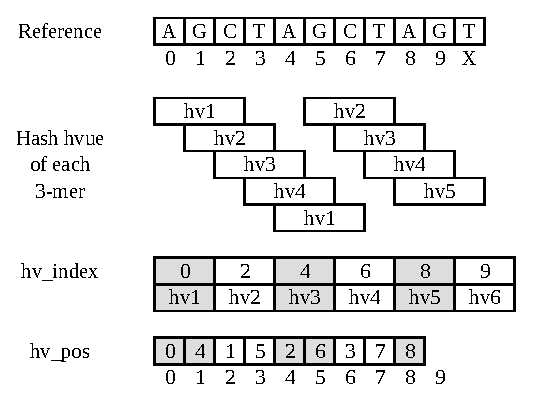
\includegraphics[width=0.9\linewidth]{HIdx}
% 		\caption{Memory layout of the hash index. For the sake of simplicity, we use 3-mers instead of 12-mers.}
% 		\label{HIdx}
% 	\end{center}
% \end{figure}

% \subsubsection{Myers Bit-Vector Algorithm}
% Myers' bit-parallel algorithm consists of a preprocessing stage and a computation stage. During preprocessing we determine the contributions of $eq_{ij}$ (see Equation~\ref{EVform}). The computation stage implements the DP algorithm in bit-vector representation. Since our alphabet contains only the four symbols 'A', 'C', 'G', and 'T', we can bit-pack both the reference and the read using 2 bits per nucleotide. Moreover, $eq_{i,j}$ can be calculated efficiently using a combination of bitshift and bit-wise compare instructions. 
% %(can also be calculated by $\lnot$ and $\oplus$ or some intrinsic).

% \subsubsection{Banded Smith-Waterman Algorithm}
% The fraction of remaining intervals passing the aforementioned filtration and verification cascade is rather small due to its high pruning power. Hence, the alignment phase accounts only for a minor portion of the overall execution time. As a result, it is sufficient to implement an off-the-shell version of the Smith-Waterman algorithm executed on the 64 SPs of a CG. We further optimize the DP algorithm to only consider cells $(i, j)$ within a band $|i - j| \leq e$ where $e$ denotes the restriction of the edit distance. Note that the time taken for the alignment phase is almost negligible (roughly 1/1000 of the verification step) and thus less worthy to optimize.
% \subsection{Myers Performance Analysis}

% Since the core computing stage is the verification stage, and it used Myers' algorithm, we also evaluated the performance of our implementation of Myers algorithm, with read length from 108 to 2048, and the performance is measured in billion cell updates per second (GCUPS).


% We use a single CG in this series of experiment, and take first chromosome of hg19 (~250 million bps) as reference, while reads are generated by Li's wgsim\cite{wgsim} with error rate 0.04 since mason does not support very longer reads. For short reads (lengths below 300), we use 1,000,000 generated sequences as input, and 100,000 sequences for longer reads, the result is shown in Table.\ref{varlenexp} and Fig.\ref{VarLenCha}, it shows that longer reads have a better GCUPS, which is mainly because we can use arbitrary length of LDM and control it manually, which avoids the issues come out when sequence is longer than a cache page, and the ratio of computation is increased.
% \begin{table}[!htb]
% 	\begin{threeparttable}
% 		\begin{tabular}{rrrrr}
% 			\hline
% 			\multicolumn{2}{c}{Reads} &
% 			\multicolumn{1}{c}{\multirow{2}{*}{Time(s)}} &
% 			\multicolumn{1}{c}{Locations}  &
% 			\multicolumn{1}{c}{\multirow{2}{*}{GCUPS}} \\\cline{1-2}
% 			\multicolumn{1}{c}{Length} &
% 			\multicolumn{1}{c}{Count} &&
% 			\multicolumn{1}{c}{Verified}\\
% 			\hline
% 			108  & 1,000,000 & 86  & 556,578,400 & 75 \\
% 			160  & 1,000,000 & 123 & 568,148,613 & 118 \\
% 			200  & 1,000,000 & 185 & 703,355,610 & 152 \\
% 			256  & 1,000,000 & 193 & 575,918,687 & 196 \\
% 			500  & 100,000 & 49   & 54,639,771  & 278\\
% 			1,280 & 100,000 & 171  & 40,924,672  & 394\\
% 			2,048 & 100,000 & 1,981 & 213,913,594 & 452\\
% 			\hline
% 		\end{tabular}
% 		\caption{Evaluation of various length reads alignment.}
% 		\label{varlenexp}
% 	\end{threeparttable}
% \end{table}

% \begin{figure}[!htb]
% 	\begin{center}
% 		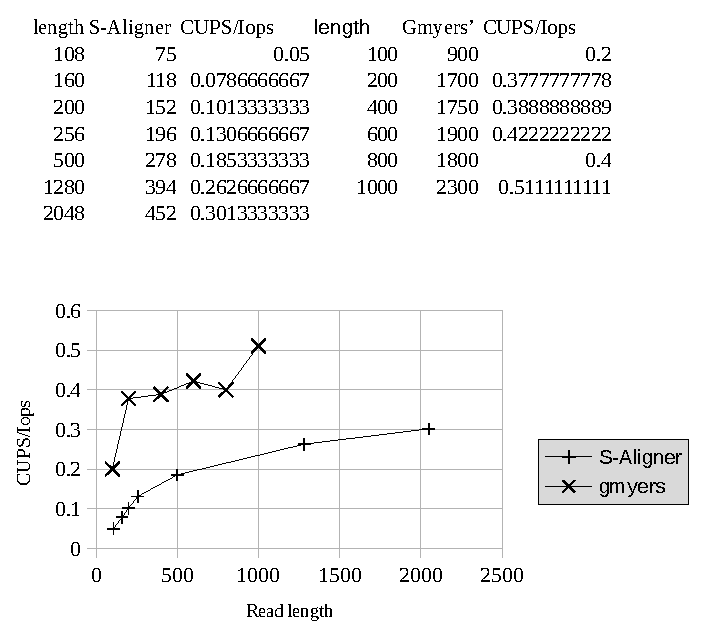
\includegraphics[width=1\linewidth]{VarLenCha}
% 		\caption{Performance of different read length}
% 		\label{VarLenCha}
% 	\end{center}
% \end{figure}

%In our experiments we process approximately 800 GB of reads on over 13,000 SW26010 nodes executing more than 50,000 dispatched processes. Thus, a na\"ive partitioning of the read file into 50,000 pieces of approximately 16 MB size is not a suitable solution due to the excessive data replication of the reference genome index. Instead,

%%\subsection{Workflow of S-Aligner}

%The second level of parallelism employs a fine-grained parallelization scheme exploiting the threading and SIMD capabilities of a CG. Our implementation within a single node is a comprehensive read mapper  based on a traditional seed-and-extend approach. with three major steps: filtration, verification and alignment. The filtration step prunes intervals uses a filter following pigeonhole principle: if the max number of allowed edits between the read and an interval is $e$, then we can divide the read to more than $e$ $q\_gram$s, and then at least one $q\_gram$ can be mapped to the candidate without any edit, this can be done easily by a hash based index which can be loaded from a preprocessed index file or alternatively calculated on-the-fly. Besides that, it stores the passing intervals in a SIMD friendly manner allowing for efficient vectorization during the subsequent verification step. Verification aims to select intervals that comply with restricted edit distance using Myers' bit-parallel algorithm. Hence, false positives from the filtration step are weeded out. Afterwards, we employ a banded Smith-Waterman algorithm to align the remaining intervals that have passed verification. Figure~\ref{FrmWk} visualizes the workflow of the intra-CG implementation.

%\begin{figure}[!htb]
	%\begin{center}
%	\includegraphics[width=1\linewidth]{FrmWk}
%	\caption{Workflow of our implementation: gray boxes correspond to tasks done by SPs.}
%	\label{FrmWk}
	%\end{center}
%\end{figure}

%\subsection{Parallelization}
%\subsubsection{Large Scale Inter-CG Parallelization}
%Furthermore, we use a rotational output strategy during the writing of results by serializing the output of four CGs within a many-core processor to overcome the aforementioned bandwidth limitations of the system interface. The overall design of our coarse-grained task partitioning and file loading strategy is depicted in Figure~\ref{TaskGrid}.
%Outgoing from the starting position of a process in the task grid, it loads its corresponding reference block and read chunk and subsequently communicates them via a broadcast to its respective row group or column group.

%Since our filtration strategy is differs from RazerS3, thus the relative speed of this two mappers are not stable, our mapper executes better on shorter reads while not so bad with longer reads.
%As we can see from the table we can achieve 3$\times$ speedup over RazerS3 while S-Aligner runs on a slower platform than RazerS3.

% \subsubsection{Comparison to BWA}
% BWA is one of the most well-known "any-best" mappers, it runs many times faster than RazerS3 on Intel platforms, but if I compile it straight forward to SW26010, since it cannot make full use of SPs, SIMD and LDM, it runs two times slower than our implementation, while finding much less locations, showing that is important to make some changes according to this specific architecture.